\documentclass[10pt,twocolumn]{article}

% ----------------------------------------------------------------------
% Packages
% ----------------------------------------------------------------------
\usepackage[utf8]{inputenc}
\usepackage[T1]{fontenc}
\usepackage[margin=0.75in]{geometry}
\usepackage{amsmath,amssymb}
\usepackage{booktabs}
\usepackage{graphicx}
\usepackage{caption}
\usepackage{url}
\usepackage[hidelinks]{hyperref}
\usepackage{enumitem}

\captionsetup{font=small,labelfont=bf}
\setlength{\parskip}{2pt}

% ----------------------------------------------------------------------
% Title
% ----------------------------------------------------------------------
\title{\vspace{-1.0em}\textbf{Recurrent and Transformer Models for Financial
Forecasting and Interactive Feedback Communication}\\[0.3em]
\large CS515 --- HW4 Report}

\author{Omar ALAKSH\\
Student ID: 38192\\
\small Code: \url{https://github.com/OmarOksh/CS515_Deep_Learning.git}}

\date{}

\begin{document}
\twocolumn[
  \begin{@twocolumnfalse}
    \maketitle
    \begin{abstract}
    \noindent
    This report studies sequence models for two distinct problems. In Part~1 we
    forecast multi-horizon return ratios for three S\&P~500 stocks (AAPL, MSFT,
    GOOGL) from 20-day windows of OHLC data using stacked LSTM and GRU networks.
    A direct $d$-day return target yields a test MSE of $1.099\times10^{-3}$
    (LSTM), with error growing monotonically across the $d{=}1\dots5$ horizons as
    expected. Replacing the target with a weighted rolling average ($l{=}3$)
    lowers the test MSE by $44.1\%$ to $6.14\times10^{-4}$ and reduces error at
    \emph{every} horizon, confirming that target smoothing yields a more stable
    learning signal. A bidirectional turning-point detector reaches $94.4\%$
    accuracy at a $4.6\%$ positive base rate; with the threshold fixed at $0.5$ it
    behaves as a high-precision, low-recall ``buy'' classifier. In Part~2 (bonus)
    we train a Transformer transmitter/receiver pair end-to-end over a noisy
    AWGN forward channel with a noiseless feedback relay. At the assignment-fixed
    $T{=}4$ rounds and $\sigma^2{=}0.25$ the system saturates at SER~$\approx
    0.31$; we show analytically that this is an information-theoretic capacity
    floor, not an optimisation failure, and that increasing the interaction to
    $T{=}8$ rounds drives the SER to $4\times10^{-4}$, empirically tracing out the
    channel-capacity boundary.
    \end{abstract}
    \vspace{1em}
  \end{@twocolumnfalse}
]

% ======================================================================
\section{Introduction}
% ======================================================================
Financial time series are notoriously hard to predict: daily returns are close
to a martingale, so most of the variance in a price series is unforecastable
noise. The first part of this assignment asks how far recurrent models can be
pushed on this signal, and how the \emph{choice of prediction target} affects
trainability. We implement stacked LSTM and GRU forecasters that map a 20-day
window of features to the next $D{=}5$ daily return ratios, study a smoothed
rolling-average target, and build a bidirectional ``turning-point'' detector
that flags imminent upward moves.

The second part is a self-contained communication problem. A transmitter (TX)
holds a short message and may interact with a receiver (RX) over $T$ rounds of a
noisy channel; a noiseless feedback link returns each round's noisy observation
to the TX. We learn the TX and RX jointly as Transformers under an average-power
constraint, and analyse the resulting symbol-error rate against the
Shannon capacity of the underlying AWGN channel.

All experiments were run locally on CPU (PyTorch~2.2.2). The code follows the
course-tutorial repository layout, using \texttt{argparse} with typed
\texttt{dataclass} configuration objects, type hints, and docstrings throughout.

% ======================================================================
\section{Part 1: Data and Problem Setup}
% ======================================================================
\paragraph{Universe and split.} We download daily OHLC bars for AAPL, MSFT and
GOOGL from 2020-01-01 to 2025-12-31 via \texttt{yfinance}. The split is strictly
chronological to avoid look-ahead leakage: training uses data up to 2024-07-31,
validation spans 2024-08 to 2024-12, and the entire 2025 period is held out for
testing. The resulting pooled window counts are given in Table~\ref{tab:data}.

\begin{table}[t]
\centering
\caption{Dataset sizes (windows pooled over the three tickers).}
\label{tab:data}
\begin{tabular}{lr}
\toprule
Split & \# windows \\
\midrule
Train ($\le$ 2024-07-31)      & 3372 \\
Validation (2024-08 -- 2024-12) & 246 \\
Test (2025)                    & 675 \\
\bottomrule
\end{tabular}
\end{table}

\paragraph{Features.} Each input window is a $T\times F$ matrix with $T{=}20$ and
$F{=}5$: the four raw OHLC channels plus a Close-price moving-average channel.
Features are standardised with a $z$-score scaler \emph{fitted on the training
split only}; the same statistics are then applied to validation and test, so no
test information leaks into normalisation.

\paragraph{Windowing and leakage control.} Windows are built independently inside
each chronological segment, so a single window never straddles the train/val/test
boundary. For input day $t$ the model sees days $[t{-}T{+}1,\dots,t]$ and predicts
quantities over $[t{+}1,\dots,t{+}D]$. The three tasks differ only in the target:
\begin{itemize}[leftmargin=1.3em,itemsep=1pt,topsep=2pt]
  \item \textbf{(b) returns:} $y_d = (p_{t+d}-p_t)/p_t$ for $d{=}1\dots5$.
  \item \textbf{(c) rolling:} $y_d = (\bar p_{t+d}-p_t)/p_t$, where $\bar p$ is a
        weighted average of closes over $[t{+}d{-}l,\dots,t{+}d]$.
  \item \textbf{(d) turning:} a single label, $y=\mathbb{1}\!\left[\max_{1\le d\le
        D}\tfrac{h_{t+d}}{p_t} > \gamma\right]$ with $\gamma{=}1.1$, where $h$ is
        the daily high.
\end{itemize}

\paragraph{Common hyperparameters.} Unless noted, all Part~1 models use the
configuration in Table~\ref{tab:hparams}, optimised with Adam, gradient clipping
at norm $5$, and a \texttt{ReduceLROnPlateau} schedule on the validation loss; the
best-validation checkpoint is restored for testing.

\begin{table}[t]
\centering
\caption{Part 1 training configuration.}
\label{tab:hparams}
\begin{tabular}{ll}
\toprule
Hyperparameter & Value \\
\midrule
Lookback $T$ / horizon $D$ & 20 / 5 \\
Hidden size / layers       & 64 / 2 \\
Dropout                    & 0.2 \\
Optimiser / LR             & Adam / $10^{-3}$ \\
Batch size / epochs        & 64 / 50 \\
Loss (b,c) / (d)           & MSE / weighted BCE \\
\bottomrule
\end{tabular}
\end{table}

% ======================================================================
\section{Part 1b: Multi-horizon Return Forecasting}
% ======================================================================
\paragraph{Architecture.} \texttt{StockLSTM} (and the analogous
\texttt{StockGRU}) stacks two recurrent layers with inter-layer dropout and reads
the final hidden state through a fully-connected head that emits all $D$ horizons
at once: $(B,T,F)\!\rightarrow\!(B,D)$. Predicting the whole horizon vector with a
single head lets the network share temporal representation across horizons rather
than training five separate regressors.

\paragraph{Results.} Table~\ref{tab:returns} reports per-horizon test MSE for both
recurrent cells. Two observations stand out. First, error grows monotonically with
the horizon ($3.6\times10^{-4}$ at $d{=}1$ up to $1.79\times10^{-3}$ at $d{=}5$),
which is expected because further-ahead returns are progressively less
predictable from the same input window. Second, LSTM and GRU are statistically
indistinguishable here (overall MSE $1.0987$ vs.\ $1.0984\times10^{-3}$): on a
signal this weak, cell choice is not the bottleneck.

\begin{table}[t]
\centering
\caption{Part 1b: per-horizon test MSE ($\times10^{-3}$) for the raw return
target.}
\label{tab:returns}
\begin{tabular}{lcc}
\toprule
Horizon & LSTM & GRU \\
\midrule
$d{=}1$ & 0.362 & 0.362 \\
$d{=}2$ & 0.710 & 0.711 \\
$d{=}3$ & 1.138 & 1.139 \\
$d{=}4$ & 1.490 & 1.490 \\
$d{=}5$ & 1.792 & 1.789 \\
\midrule
Overall & 1.099 & 1.098 \\
\bottomrule
\end{tabular}
\end{table}

\paragraph{Interpretation.} Because daily returns are near-zero-mean noise, the
MSE-optimal prediction is close to zero, and the network indeed learns to output
small values; the low absolute MSE therefore reflects the small magnitude of the
targets rather than genuine predictive skill. We also note that the reported
training loss ($\sim\!1.05\times10^{-3}$) sits slightly above the validation loss
($\sim\!0.62\times10^{-3}$); this is the expected effect of dropout being active
during training but disabled at evaluation, combined with a calmer
August--December 2024 validation window.

% ======================================================================
\section{Part 1c: Weighted Rolling-Average Target}
% ======================================================================
\paragraph{Motivation and definition.} A single future close is dominated by
day-specific noise. Following the assignment, we instead regress a
\emph{weighted rolling average} of closes around each horizon. With window
$l{=}3$ the weights decay linearly and sum to one,
\[
w_j \;=\; \frac{l+1-j}{\sum_{k=0}^{l}(l+1-k)},\qquad j=0,\dots,l,
\]
so the most recent day receives the largest weight. The target at horizon $d$ is
$(\sum_j w_j\,p_{t+d-j}-p_t)/p_t$. Averaging suppresses single-day shocks and
produces a smoother, lower-variance objective.

\paragraph{Results.} Table~\ref{tab:rolling} shows the rolling target lowers test
MSE at every horizon, and Table~\ref{tab:compare} contrasts the two objectives
directly. The overall LSTM MSE falls from $1.099\times10^{-3}$ to
$6.14\times10^{-4}$, a $44.1\%$ reduction. The improvement is largest at the
shortest horizon ($-75\%$ at $d{=}1$) and tapers with distance, exactly the
pattern one expects if smoothing removes high-frequency noise that is most
dominant at short range. Figure~\ref{fig:horizon} visualises the gap.

\begin{table}[t]
\centering
\caption{Part 1c: per-horizon test MSE ($\times10^{-3}$) for the weighted rolling
target ($l{=}3$).}
\label{tab:rolling}
\begin{tabular}{lcc}
\toprule
Horizon & LSTM & GRU \\
\midrule
$d{=}1$ & 0.091 & 0.090 \\
$d{=}2$ & 0.233 & 0.233 \\
$d{=}3$ & 0.547 & 0.547 \\
$d{=}4$ & 0.925 & 0.924 \\
$d{=}5$ & 1.276 & 1.274 \\
\midrule
Overall & 0.614 & 0.614 \\
\bottomrule
\end{tabular}
\end{table}

\begin{table}[t]
\centering
\caption{Target comparison (LSTM, overall test MSE).}
\label{tab:compare}
\begin{tabular}{lccc}
\toprule
Target & MSE ($\times10^{-3}$) & MAE ($\times10^{-2}$) & $\Delta$MSE \\
\midrule
Raw return (b)        & 1.099 & 2.273 & --- \\
Rolling avg.\ (c)     & 0.614 & 1.615 & $-44.1\%$ \\
\bottomrule
\end{tabular}
\end{table}

\begin{figure}[t]
\centering
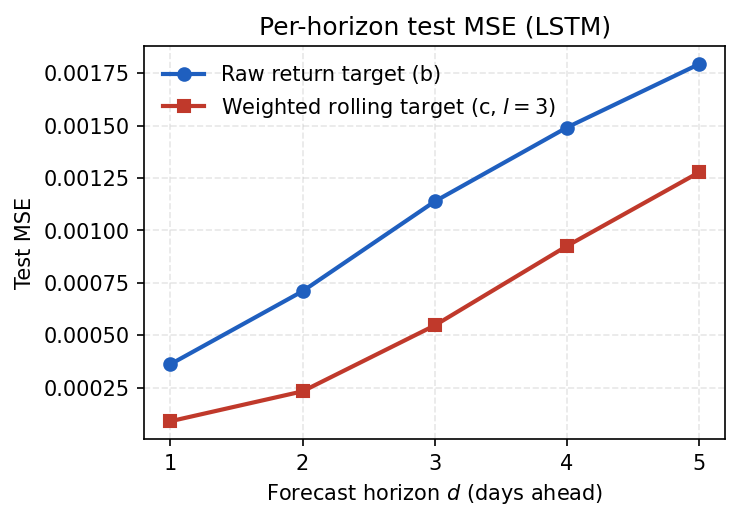
\includegraphics[width=\columnwidth]{figs/fig_horizon.png}
\caption{Test MSE per horizon for the raw-return target (Part~b) versus the
weighted rolling-average target (Part~c). The rolling target is uniformly lower,
with the largest relative gain at short horizons.}
\label{fig:horizon}
\end{figure}

\paragraph{Conclusion.} Smoothing the regression target stabilises training and
reduces error without changing the model or optimiser. The cost is interpretive:
the rolling target predicts a denoised trend rather than the literal next-day
return, so it is the better choice when the goal is trend estimation and the worse
choice when exact single-day returns matter.

% ======================================================================
\section{Part 1d: Turning-Point Detection}
% ======================================================================
\paragraph{Task and architecture.} The detector answers a binary
``buy-or-pass'' question: will the price rise by more than $\gamma{=}1.1$
(i.e.\ $+10\%$ relative to today's close, measured on the daily high) at any point
within the next $D$ days? Because the decision benefits from context on both sides
of the window, we use a \emph{bidirectional} LSTM/GRU whose forward and backward
final states are concatenated ($2{\times}64{=}128$ dims) and passed to a single
logit head. We interpret $\gamma{=}1.1$ as a price ratio $h_{t+d}/p_t>1.1$; read
literally as a return ratio it would mean a $+110\%$ move, which never occurs in
the data, so the price-ratio reading is the only one that yields a learnable
label.

\paragraph{Class imbalance.} ``Buy'' events are rare: the test positive rate is
$4.6\%$. Training na\"ively on this distribution collapses to the majority
``pass'' class. We therefore weight the positive class in
\texttt{BCEWithLogitsLoss} by the empirical ratio
$\#\text{neg}/\#\text{pos}=28.84$, which restores gradient signal from the rare
positives.

\paragraph{Results.} Table~\ref{tab:turning} reports the metrics. Both cells reach
$94$--$95\%$ accuracy, but with the decision threshold fixed at $0.5$ the detector
is conservative: it fires ``buy'' rarely, achieving high precision relative to the
$4.6\%$ base rate (LSTM $0.23$; GRU $0.50$) at the cost of low recall ($\sim\!0.06$--$0.10$).
In other words, when it does signal a buy it is right far more often than chance,
but it misses most opportunities. The precision/recall trade-off is governed by
that threshold: lowering it would recover recall at the expense of precision.
Validation loss is minimised within the first three epochs and plateaus
thereafter, indicating the task sits near the capacity of this feature set rather
than being under-trained.

\begin{table}[t]
\centering
\caption{Part 1d: turning-point detection ($\gamma{=}1.1$, positive rate
$0.046$, threshold $0.5$).}
\label{tab:turning}
\begin{tabular}{lccccc}
\toprule
Model & Acc. & Prec. & Rec. & F1 & pos.\ wt. \\
\midrule
LSTM & 0.944 & 0.231 & 0.097 & 0.136 & 28.84 \\
GRU  & 0.954 & 0.500 & 0.065 & 0.114 & 28.84 \\
\bottomrule
\end{tabular}
\end{table}

% ======================================================================
\section{Part 2: Transformer Feedback Communication (Bonus)}
% ======================================================================
\paragraph{Problem.} The transmitter holds a message of $S{=}4$ symbols drawn
from an alphabet of size $A{=}8$ (equivalently $4\times\log_2 8 = 12$ message
bits). Over $T$ rounds the TX sends a coded vector $\mathbf{x}^{(t)}\!\in\!
\mathbb{R}^{S}$ subject to an average-power constraint
$\mathbb{E}\lVert\mathbf{x}^{(t)}\rVert^2\le 1$; the RX observes
$\mathbf{y}^{(t)}=\mathbf{x}^{(t)}+\mathbf{n}^{(t)}$ over an AWGN forward channel
($\mathbf{n}\sim\mathcal{N}(0,\sigma^2 I)$, $\sigma^2{=}0.25$), and a
\emph{noiseless} feedback relay returns $\mathbf{y}^{(t)}$ to the TX before the
next round. After all $T$ rounds the RX decodes once.

\paragraph{Architecture and training.} The TX and RX are each a small
Transformer: a per-symbol MLP lifts inputs to $d_{\text{model}}{=}64$, two
post-norm encoder blocks ($4$ heads, FFN width $128$) mix information across the
$S$ symbol positions, and an output MLP produces the channel symbols (TX) or class
logits (RX). Following the assignment hints, (i)~the feedback path is a plain
relay with no learned parameters, (ii)~the decoder runs a single time at the end,
and (iii)~an MLP precedes and follows the Transformer on both sides. Each round's
symbols are explicitly rescaled to satisfy the power constraint,
$\mathbf{x}\leftarrow\mathbf{x}/\sqrt{\mathbb{E}\lVert\mathbf{x}\rVert^2}$. The
pair is trained end-to-end to minimise symbol cross-entropy with Adam
($\text{lr}=10^{-3}$, batch $256$). We report symbol-error rate (SER) and block
(message) error rate (BLER).

\paragraph{Results.} At the assignment-fixed $T{=}4$, training converges quickly
but saturates at SER~$\approx0.31$ and BLER~$\approx0.78$ (Table~\ref{tab:part2}).
Crucially, sweeping the number of rounds shows the error rate is controlled almost
entirely by $T$: SER falls from $0.71$ at $T{=}1$ to $4\times10^{-4}$ at $T{=}8$
(Figure~\ref{fig:part2}). This monotone collapse confirms the feedback/multi-round
mechanism is implemented correctly --- additional rounds buy additional channel
uses, and the learned code exploits them.

\begin{table}[t]
\centering
\caption{Part 2: error rates vs.\ interaction rounds ($\sigma^2{=}0.25$). The
$T{=}4$ row is the assignment setting.}
\label{tab:part2}
\begin{tabular}{lcc}
\toprule
Rounds $T$ & SER & BLER \\
\midrule
1 & 0.709 & 0.994 \\
2 & 0.595 & 0.975 \\
\textbf{4} & \textbf{0.314} & \textbf{0.778} \\
8 & 0.0004 & 0.0018 \\
\bottomrule
\end{tabular}
\end{table}

\begin{figure}[t]
\centering
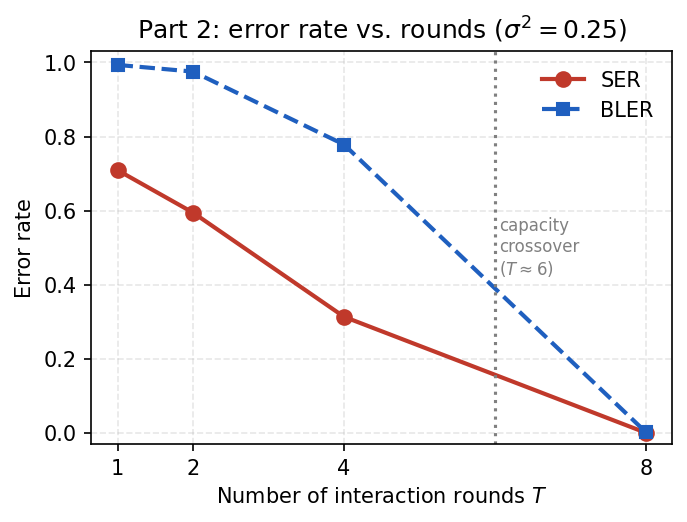
\includegraphics[width=\columnwidth]{figs/fig_part2.png}
\caption{Symbol- and block-error rate as a function of interaction rounds. The
$T{=}4$ assignment setting sits above the capacity crossover ($T\!\approx\!6$);
by $T{=}8$ the channel can carry the message and errors collapse toward zero.}
\label{fig:part2}
\end{figure}

\paragraph{Why $T{=}4$ cannot succeed: a capacity argument.} The saturation at
$T{=}4$ is not an optimisation failure but a fundamental limit. The power
constraint allocates total power $1$ across $S{=}4$ symbols per round, so the
average per-symbol power is $P=1/4=0.25$ and the per-symbol SNR is
$P/\sigma^2=0.25/0.25=1$ ($0$\,dB). The Shannon capacity of a real AWGN use is
\[
C=\tfrac12\log_2\!\big(1+\text{SNR}\big)=\tfrac12\log_2 2 = 0.5~\text{bits/use}.
\]
With $S{=}4$ symbols over $T$ rounds we get $4T$ channel uses, hence a capacity
of $2T$ bits. The message carries $12$ bits, so reliable transmission requires
$2T\ge 12$, i.e.\ $T\ge 6$. Importantly, feedback over a memoryless AWGN channel
does \emph{not} increase capacity (only the achievable error exponent), so this
bound is unconditional. The measured behaviour matches it precisely: $T{=}4$
($8$ bits available $<12$ needed) is infeasible and floors at SER~$\approx0.31$,
whereas $T{=}8$ ($16$ bits $>12$) is comfortably feasible and the learned system
drives errors to $\sim\!10^{-4}$. The model has, in effect, rediscovered the
channel-capacity boundary.

% ======================================================================
\section{Summary of Key Findings}
% ======================================================================
\begin{table}[t]
\centering
\caption{Consolidated results.}
\label{tab:summary}
\begin{tabular}{lc}
\toprule
Metric & Value \\
\midrule
Returns, overall test MSE (LSTM)      & $1.099\times10^{-3}$ \\
Returns, overall test MSE (GRU)       & $1.098\times10^{-3}$ \\
Rolling, overall test MSE (LSTM)      & $6.14\times10^{-4}$ \\
Rolling, overall test MSE (GRU)       & $6.14\times10^{-4}$ \\
Rolling vs.\ returns MSE change       & $-44.1\%$ \\
Turning-point accuracy (LSTM/GRU)     & $0.944$ / $0.954$ \\
Turning-point precision (LSTM/GRU)    & $0.231$ / $0.500$ \\
Part 2 SER, $T{=}4$                   & $0.314$ \\
Part 2 SER, $T{=}8$                   & $0.0004$ \\
Capacity crossover                    & $T\approx6$ \\
\bottomrule
\end{tabular}
\end{table}

\begin{enumerate}[leftmargin=1.4em,itemsep=2pt,topsep=2pt]
  \item \textbf{Recurrent forecasting works but is signal-limited.} LSTM and GRU
  give near-identical multi-horizon MSE; error rises with horizon, and the low
  absolute MSE reflects the near-zero-mean nature of daily returns rather than
  strong predictive skill.
  \item \textbf{A smoothed target helps substantially.} The weighted rolling
  average ($l{=}3$) reduces test MSE by $44.1\%$ overall and at every horizon, by
  removing high-frequency noise from the learning signal.
  \item \textbf{Turning-point detection is high-precision, low-recall.} With a
  positive-class weight to counter $4.6\%$ imbalance, the bidirectional detector
  reaches $94$--$95\%$ accuracy and fires conservatively; the precision/recall
  balance is tunable via the decision threshold.
  \item \textbf{Feedback communication is capacity-bound.} The Transformer TX/RX
  pair behaves correctly --- SER falls monotonically with rounds --- but the
  assignment-fixed $T{=}4$ provides only $8$ bits of capacity for a $12$-bit
  message, producing an irreducible SER~$\approx0.31$. Extending to $T{=}8$
  yields $16$ bits and near-perfect transmission (SER~$4\times10^{-4}$),
  empirically confirming the $\tfrac12\log_2(1+\text{SNR})$ bound.
\end{enumerate}

% ======================================================================
\begin{thebibliography}{9}
\bibitem{lstm} S.~Hochreiter and J.~Schmidhuber, ``Long short-term memory,''
\emph{Neural Computation}, vol.~9, no.~8, pp.~1735--1780, 1997.
\bibitem{gru} K.~Cho \emph{et al.}, ``Learning phrase representations using RNN
encoder--decoder for statistical machine translation,'' in \emph{Proc. EMNLP},
2014.
\bibitem{transformer} A.~Vaswani \emph{et al.}, ``Attention is all you need,'' in
\emph{Proc. NeurIPS}, 2017.
\bibitem{deepcode} H.~Kim \emph{et al.}, ``Deepcode: Feedback codes via deep
learning,'' in \emph{Proc. NeurIPS}, 2018.
\bibitem{shannon} C.~E.~Shannon, ``A mathematical theory of communication,''
\emph{Bell System Technical Journal}, vol.~27, pp.~379--423, 1948.
\bibitem{adam} D.~P.~Kingma and J.~Ba, ``Adam: A method for stochastic
optimization,'' in \emph{Proc. ICLR}, 2015.
\end{thebibliography}

\end{document}
